\DiaryEntry{Gamma Function}{2015-07-27}{Maths}

\subsection{Partial Integration}

First thing is the derivation of the partial integration: We differentiate the product of two functions

\bee
\frac{d (u(x)v(x)}{dx} = u(x) \frac{d v(x)}{dx} + v(x) \frac{d u(x)}{dx}
\eee
%
integrate both sides

\bee
u(x)v(x) = \int u(x) \frac{d v(x)}{dx} dx + \int v(x) \frac{d u(x)}{dx} dx
\eee
%
and rearrange the result so that we obtain
%
\bee
\int u(x) \frac{d v(x)}{dx} dx = u(x)v(x) - \int v(x) \frac{d u(x)}{dx} dx
\eee
%
or - in a more sloppy notation - we have
%
\bee
\int u v' dx = uv - \int u' v dx
\eee

\subsection{Definition and Properties}

The Gamma function $\Gamma(x)$ is defined according to
%
\bee
\Gamma(x) = \int_0^\infty t^{x-1}e^{-t} dt
\eee
%
and fulfills the following recurrence relation
%
\bee
\Gamma(x+1) = x \Gamma(x)
\eee
%
which we can prove as follows
%
\bee
\Gamma(x+1) = \int_0^\infty t^{x}e^{-t} dt
\eee
by partial integration ($v'e^{-t} \rightarrow v = -e^{-t}, u=t^x \rightarrow u'=x t^{x-1}$) we obtain
%
\bee
\Gamma(x+1) = \left. -t^x e^{-t} \right|_0^\infty - \int_0^\infty x t^{x-1}(-1)e^{-t} dt = 0 + \int_0^\infty x t^{x-1}e^{-t} dt = x \int_0^\infty t^{x-1}e^{-t} dt
\eee
%
where in the last step we have used the fact that the integral is over $t$ and therefore $x$ can be taken out of the integral. Comparing with the definition, we see that
%
\bee
\Gamma(x+1) = x \Gamma(x) \qed
\eee
%
Next we calculate the value of $\Gamma(1)$ as
%
\bee
\Gamma(1) = \int_0^\infty t^{0}e^{-t} dt = \int_0^\infty e^{-t} dt = \left. e^{-t} \right|_0^\infty = 1
\eee
%
The function plot looks as follows (be careful; Julia uses a gamma function shifted by one):

\begin{figure}[hbt!]
\centering
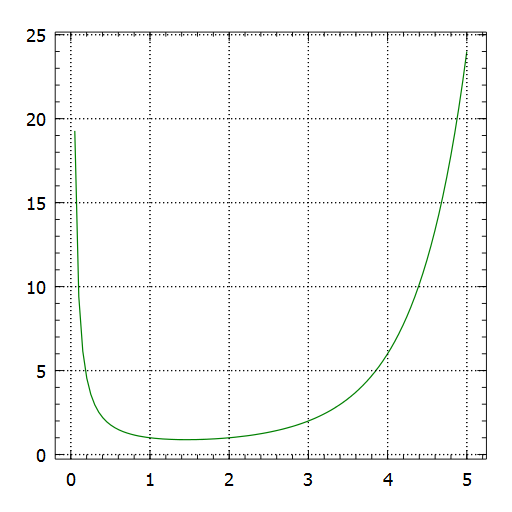
\includegraphics[scale=0.5]{images/gamma_plot.png}
\end{figure}
